\documentclass[12pt]{article}
\usepackage[T1]{fontenc}
\usepackage[utf8]{inputenc}
\usepackage{lmodern}         % recommended
\usepackage{newunicodechar}
\usepackage[croatian]{babel}
\usepackage{amsmath}
\usepackage{graphicx}
\usepackage{hyperref}
\usepackage{listings}
\usepackage{listings}
\usepackage{color} % For coloring code (optional)
\usepackage{tikz}
\usetikzlibrary{arrows}
\usetikzlibrary{automata, positioning}
\usepackage{xcolor}
\usepackage{listingsutf8}


\lstset{
	language=Matlab,
	basicstyle=\ttfamily,
	breaklines=true,
	keywordstyle=\color{blue},
	stringstyle=\color{red},
	commentstyle=\color{green},
	morecomment=[l][\color{magenta}]{\#},
	columns=fullflexible,
	xleftmargin=0pt,
	framexleftmargin=0pt,
	resetmargins=true,
	backgroundcolor=\color{gray!20},
	frame=single,
	framesep=10pt,
	framerule=0pt,
	inputencoding=utf8, % Set UTF-8 encoding
	extendedchars=true, % Enable extended characters
	literate= % Define conversions for special characters
	{č}{{\v{c}}}1
	{ć}{{\'{c}}}1
	{đ}{{\dj{}}}1
	{š}{{\v{s}}}1
	{ž}{{\v{z}}}1
	{Č}{{\v{C}}}1
	{Ć}{{\'{C}}}1
	{Đ}{{\DJ{}}}1
	{Š}{{\v{S}}}1
	{Ž}{{\v{Z}}}1
}



\title{Izvještaj: Laboratorijska vježba za skrivene Markovljeve modele}
\author{Dominik Barukčić}
\date{\today}

\begin{document}
	
	\maketitle
	
	% MATLAB Kod
%	\subsubsection*{MATLAB Kod}
%	\begin{lstlisting}
%		
%		a = 10;
%		b = 20;
%		c = a + b;
%		disp(c);
%	\end{lstlisting}
%	
%	% Rezultati
%	\subsubsection*{Rezultati}
%	Ovdje navedite rezultate izvršavanja koda.
%	
%	% IZVJEŠTAJ
%	\subsubsection*{IZVJEŠTAJ}
%	Ovdje odgovorite na pitanja, komentirajte rezultate, i sl. ovisno o tekstu pod-zadatka.
	
	
	
	\section{Opis eksperimenta}
	Odabrani stohastički eksperiment je temeljen na bacanju tri pristrane igrače kocke s mogućim ishodima bacanja od 1 do 6. Ove kocke su „podešene“ na način da će prva kocka u prosjeku, u pola svih bacanja dati broj „1“, da će druga kocka također u pola svih bacanja dati broj „3“ i da će treća na jednak način u pola svih bacanja dati broj „5“. Vjerojatnosti preostalih ishoda bacanja bitno su manje, ali nisu jednake, nego su ovisne o pojedinoj kocki za svaki od preostalih 5 mogućih brojeva. Ishod bacanja kocke vidljiv je gledateljima, dok ono što im nije vidljivo jest informacija koja od tri pristrane kocke je korištena pri pojedinom bacanju, pa stoga indeks korištene kocke (1., 2. ili 3. kocka) predstavlja skriveno stanje ovog modela.
	
	Promjene skrivenih stanja definirane su prijelaznom matricom modela, pri čemu neki prijelazi u ovom eksperimentu nisu dozvoljeni, tj. imaju nultu vjerojatnost. Konkretno, ako je u aktualnom bacanju korištena prva kocka, tada će u narednom bacanju biti korištena ta ista kocka, ili druga kocka, ali ne može biti odabrana treća kocka. Analogno, ako je model u stanju bacanja druge kocke, može ostati u tom stanju, ili prijeći u stanje treće kocke, ali se ne može vratiti u stanje prve kocke. Konačno kada uđe u stanje treće kocke, može ciklički prijeći u stanje prve kocke, ili ostati u postojećem stanju, ali se ne može vratiti u stanje druge kocke. Zaključno, ovaj model nužno ciklički prolazi kroz skrivena stanja 1->2->3->1, uz mogućnost zadržavanja u aktualnom stanju. Vjerojatnost zadržavanja istog stanja iznosi (M-1)/M, dok vjerojatnost prijelaza u naredno cikličko stanje iznosi 1/M.
	
	\begin{center}
		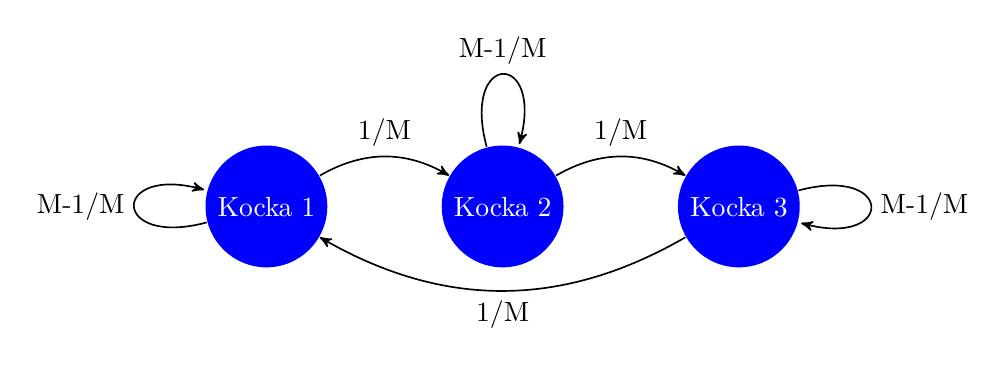
\begin{tikzpicture}[->, >=stealth', auto, semithick, node distance=3cm]
			\tikzstyle{every state}=[fill=blue,draw=none,text=white]
			
			\node[state] (A) {Kocka 1};
			\node[state] (B)[right of=A] {Kocka 2};
			\node[state] (C)[right of=B] {Kocka 3};
			
			\path
			(A) edge[bend left] node[above] {1/M} (B)
			edge[loop left] node {M-1/M} (A)
			(B) edge[bend left] node[above] {1/M} (C)
			edge[loop above] node {M-1/M} (B)
			(C) edge[bend left] node[below] {1/M} (A)
			edge[loop right] node {M-1/M} (C);
		\end{tikzpicture}
	\end{center}
	
	U svrhu definiranja početnog stanja ovog modela, dakle samo za prvo bacanje, koristi se dodatna nepristrana kocka na ovaj način: ako je ishod bacanja te nepristrane kocke „1“ za prvo bacanje će se koristiti prva pristrana kocka, za ishode „2“ ili „3“ koristit će se druga kocka, dok se u slučaju preostala tri ishoda, „4“, „5“ i „6“, kao prva baca treća pristrana kocka.
	
	\section{Opis zadanog modela}
	Slučajni eksperiment kojeg koristimo za ovu vježbu odnosi se na bacanje tri pristrane igrače kocke, gdje indeks korištene kocke predstavlja skriveno stanje ovog HMM modela. Vjerojatnosti pojedinih ishoda bacanja su različite za svaku pristranu kocku, a vjerojatnosti cikličke izmjene stanja su određene parametrom M. Za detaljni opis eksperimenta svakako pogledajte opis vježbe u ranije navedenom dokumentu.
	
	Zadani parametar zadržavanja istog stanja iznosi M=5.
	
	Matrica prijelaznih i početnih vjerojatnosti HMM modela zadane su kao:
	
	\begin{equation}
		A = \begin{bmatrix}
			4/5 & 1/5 & 0 \\
			0 & 4/5 & 1/5 \\
			1/5 & 0 & 4/5
		\end{bmatrix}
	\end{equation}
	
	
	\begin{equation}
		P = \begin{bmatrix}
			1/6 \\
			1/3 \\
			1/2
		\end{bmatrix}
	\end{equation}
	
	
	Prosječne učestalosti osmatranja pojedinih ishoda "1" do "6" za sve tri kocke u 40 bacanja su:
	
	\begin{equation}
		B\_count =\begin{bmatrix}
			20 & 4 & 5 & 2 & 4 & 5 \\
			5  & 4 & 20 & 5 & 3 & 3 \\
			1  & 2 & 5 & 7 & 20 & 5
		\end{bmatrix}
	\end{equation}
	
	
	\section{Pod-zadaci}
	
	\subsection{Pod-zadatak 1: Definiranje HMM Modela}
		% Tekst zadatka
	Temeljem zadanih ucestalosti pojedinih ishoda bacanja pristranih kocki i temeljem zadanog parametra M u vasem Moodle zadatku,
	potrebno je dopuniti predlozak Matlab skripte kako bi cjelovito opisali zadani HMM model ovog eksperimenta ukljucujuci i matricu
	vjerojatnosti osmatranja izlaznih simbola.
	
	% MATLAB Kod
	\subsubsection*{MATLAB Kod}
	\begin{lstlisting}
clear;
pack;
addpath(genpath('/Users/dominik/Desktop/Obrada informacija/Lab3/HMMall'))

% Zadani parametar zadrzavanja istog stanja M
m = 5;           

% matrica pocetnih vjerojatnosti, P
prior0=[    
1/6
1/3
1/2                 
];

% matrica vjerojatnosti prijelaza stanja, A
transmat0=[
4/5 1/5 0
0   4/5 1/5            
1/5 0   4/5
];

Q=size(prior0,1);

% Prosjecne ucestalosti osmatranja pojedinih ishoda "1" do "6" za sve tri kocke u 40 bacanja
B_count = [
20  4   5   2   4   5
5   4   20  5   3   3
1   2   5   7   20  5            
];

br_bacanja = 40;

% matrica vjerojatnosti osmatranja izlaznih simbola
obsmat0 = B_count ./ br_bacanja;
O=size(obsmat0,2);
	\end{lstlisting}
	
	\subsection{Pod-zadatak 2: Log-Izvjesnosti Osmotrenih Nizova}
	Osmotrena su dva niza duljine T=41 simbola kojeg je generirao model L:\newline
	O = [o1 .. oT] = \newline
	[ 3 6 6 4 5 1 2 3 5 4 4 5 5 3 1 6 1 5 3 5 5 5 4 5 5 5 6 5 1 6 1 3 3 3 3 3 6 3 4 1 3]\newline 
	[ 2 2 3 5 3 6 3 4 4 4 4 1 4 6 1 4 2 6 4 1 4 3 2 5 6 6 6 4 6 6 2 6 6 3 4 4 4 2 3 4 2]\newline
	(2a) Izračunajte log-izvjesnosti osmatranja ova dva niza uz zadane parametre HMM modela te ih upišite u naredna dva polja:
	
	\subsubsection*{MATLAB Kod}
	\begin{lstlisting}
fprintf('2a zadatak\n')
% dva niza duljine T simbola kojeg je generirao model L
T = 41;          
o1 = [ 3 6 6 4 5 1 2 3 5 4 4 5 5 3 1 6 1 5 3 5 5 5 4 5 5 5 6 5 1 6 1 3 3 3 3 3 6 3 4 1 3];           
o2 = [ 2 2 3 5 3 6 3 4 4 4 4 1 4 6 1 4 2 6 4 1 4 3 2 5 6 6 6 4 6 6 2 6 6 3 4 4 4 2 3 4 2];           

data = o1;
ll1 = dhmm_logprob(data, prior0, transmat0, obsmat0);
disp(ll1)

data = o2;
ll2 = dhmm_logprob(data, prior0, transmat0, obsmat0);
disp(ll2);
	\end{lstlisting}
	
	% Rezultati
	\subsubsection*{Rezultati}
	\begin{verbatim}
		2a zadatak
		-64.7879
		
		-84.4789
	\end{verbatim}
	
	(2b) Izračunajte i upišite u Moodle koliko puta je drugi niz manje izvjestan od prvog u eksponencijalnom zapisu:
	
	% MATLAB Kod
	\subsubsection*{MATLAB Kod}
	\begin{lstlisting}
fprintf('2b zadatak\n')

% izracunaj razliku log-izvjesnosti
log_prob_diff = ll1 - ll2;

% izracunaj omjer u exp obliku
prob_ratio = exp(log_prob_diff);

% koliko puta je drugi niz manje izvjestan od prvog u eksponencijalnom zapisu
fprintf('Probability ratio (o2 is less likely than o1 by): %e times\n', prob_ratio);
	\end{lstlisting}
	
	% Rezultati
	\subsubsection*{Rezultati}
	\begin{verbatim}
		2b zadatak
		Probability ratio (o2 is less likely than o1 by): 3.562017e+08 times
	\end{verbatim}
	
	% IZVJEŠTAJ
	\subsubsection*{IZVJEŠTAJ}
	Analizom omjera log-izvjesnosti možemo zaključiti da je prvi niz vjerojatniji od drugog niza, budući da je omjer veći od 1. Drugim riječima, prvi niz sadrži simbole koji imaju veću vjerojatnost prema opservacijskoj matrici, dok drugi niz uključuje simbole s manjim vjerojatnostima.
	
	\subsection{Pod-zadatak 3: Vjerojatnosti Unaprijed i Unazad}
	Za prvu sekvencu iz pod-zadatka 2 potrebno je primijeniti algoritme "Unaprijed" i "Unazad" i izračunati unaprijedne vjerojatnosti $\alpha$ i unazadne vjerojatnosti $\beta$ za sve trenutke osmatranja t=1 ... T za zadani model L.
	
	Važno: pri pozivu funkcije ne smijete aktivirati skaliranje vjerojatnosti, tj. u pozivu funkcije morate definirati ..., 'scaled', 0); kao što je učinjeno i u primjeru u uputama.
	
	Upišite koji iznos unaprijedne vjerojatnosti $\alpha$(3) ste dobili za t=26 u prvo polje, odnosno iznos unazadne vjerojatnosti $\beta$(3) za t=11 u drugo polje u eksponencijalnom zapisu.
	
	% MATLAB Kod
	\subsubsection*{MATLAB Kod}
	\begin{lstlisting}
fprintf('3. zadatak\n')      

data = o1;
data2 = o2;
if ~iscell(data)
data = num2cell(data, 2);
data2 = num2cell(data2, 2);
end
ncases = length(data);

% Forward algorithm
loglik = 0;
errors = [];
for m=1:ncases
obslik0 = multinomial_prob(data{m}, obsmat0);
obslik1 = multinomial_prob(data2{m}, obsmat0);
[alpha, beta, gamma, ll] = ...
fwdback(prior0, transmat0, obslik0, 'scaled', 0); 
if ll==-inf
errors = [errors m];
end
loglik = loglik + ll;
end

% Backward algorithm
% beta = zeros(T, length(prior0)); % Initialize beta matrix
% beta(T, :) = 1; % Initial step
% 
% for t = T-1:-1:1
%     for i = 1:length(prior0)
%         beta(t, i) = sum(transmat0(i, :) .* obsmat0(:, o1(t+1))' .* beta(t+1, :));
%     end
% end

% Display the requested probabilities
fprintf('Forward probability alpha_t(3) at t=26: %e\n', alpha(3, 26));
fprintf('Backward probability beta_t(3) at t=11: %e\n', beta(3, 11));
	\end{lstlisting}
	
	% Rezultati
	\subsubsection*{Rezultati}
	\begin{verbatim}
		Forward probability alpha_t(3) at t=26: 4.424103e-19
		Backward probability beta_t(3) at t=11: 9.854075e-20
	\end{verbatim}
	
	% IZVJEŠTAJ
	\subsubsection*{IZVJEŠTAJ}
	Unaprijedna vrijednost $\alpha$t(i) predstavlja izvjesnost cijelog niza u stanju i u vremenu T, što je ekvivalentno zadnjem koraku. S druge strane, unazadna vrijednost $\beta$1(i) odnosi se na izvjesnost cijelog niza u stanju i u prvom koraku, tj. kada t=1. Oba ova skupa vrijednosti možemo iskoristiti kako bismo izračunali log-izvjesnost cijelog niza za to određeno skriveno stanje.
	
	Formule za izračun log-izvjesnosti za određena stanja izgledaju kao logaritam $\alpha$t(i) ili logaritam $\beta$t(i), dok bismo, ako želimo izračunati izvjesnost cijelog niza za sva stanja, koristili logaritam suma $\alpha$ svih stanja u vremenu T ili logaritam izraza za terminaciju, što predstavlja log-izvjesnost izračunanu preko odgovarajuće funkcije.
	
	\subsection{Pod-zadatak 4: Dekodiranje Skrivenih Stanja}
	Potrebno je primjenom Viterbi algoritma odrediti najizvjesniji niz skrivenih stanja modela za prvi promatrani niz iz drugog podzadatka. U narednih šest polja upišite dekodirana stanja modela za prva tri i zadnja tri vremenska koraka prve opservacije:
	
	% MATLAB Kod
	\subsubsection*{MATLAB Kod}
	\begin{lstlisting}
fprintf('4. zadatak\n')     
% Najizvjesniji put
vpath = viterbi_path(prior0, transmat0, obslik0);
disp(vpath)
	\end{lstlisting}
	
	% Rezultati
	\subsubsection*{Rezultati}
	\begin{verbatim}
		4. zadatak
		Columns 1 through 17
		
		3 3 3 3 3  1    1     2     3     3     3     3     3     1   1   1   1
		
		Columns 18 through 34
		
		1 2 3 3 3  3    3     3     3     3     3     1     1     1   2   2   2
		
		Columns 35 through 41
		
		2     2     2     2     2     2     2
	\end{verbatim}
	
	\subsection{Pod-zadatak 5: Log-Izvjesnosti duž Viterbi Puta}
	Ponovite određivanje Viterbi niza stanja za drugi promatrani niz iz pod-zadatka 2. Za oba niza izračunajte log-izvjesnosti promatranja, ali samo duž dekodiranih 'optimalnih' Viterbi puteva. Usporedite dobivene rezultate s onima iz pod-zadatka 2, gdje je izračunata ukupna log-izvjesnost za sve moguće puteve skrivenih stanja. U donjim dva polja upišite razliku između log-izvjesnosti preko svih puteva i log-izvjesnosti duž Viterbi puta za oba promatrana niza:
	
	% MATLAB Kod
	\subsubsection*{MATLAB Kod}
	\begin{lstlisting}
fprintf('5. zadatak\n')          
vpath1 = viterbi_path(prior0, transmat0, obslik0);
vpath2 = viterbi_path(prior0, transmat0, obslik1);

[ll_viterbi1, p1] = dhmm_logprob_path(prior0, transmat0, obslik0, vpath1);
[ll_viterbi2, p2] = dhmm_logprob_path(prior0, transmat0, obslik1, vpath2);

% Usporedba s ukupnim log-izvjesnostima
razlika1 = ll1 - ll_viterbi1;
razlika2 = ll2 - ll_viterbi2;

fprintf('Razlika log-izvjesnosti za prvi niz (ukupno - Viterbi): %f\n', razlika1);
fprintf('Razlika log-izvjesnosti za drugi niz (ukupno - Viterbi): %f\n', razlika2);
	\end{lstlisting}
	
	% Rezultati
	\subsubsection*{Rezultati}
	\begin{verbatim}
		5. zadatak
		Razlika log-izvjesnosti za prvi niz (ukupno - Viterbi): 6.132279
		Razlika log-izvjesnosti za drugi niz (ukupno - Viterbi): 8.526175
	\end{verbatim}
	
	% IZVJEŠTAJ
	\subsubsection*{IZVJEŠTAJ}
	Primjećujemo da razlika u izvjesnosti niza preko svih stanja premašuje izvjesnost koju dobivamo putem optimalnog puta, što nam sugerira pozitivan predznak. Vjerojatno je razlog tome što izvjesnost niza preko svih stanja, za razliku od izvjesnosti putem optimalnog puta, uključuje izvjesnosti svih stanja u svakom koraku, dok putem optimalnog puta uzimamo u obzir samo najizvjesnije izvjesnosti. Ova razlika nam pruža uvid u koliko se različiti putevi razlikuju po izvjesnosti.
	
	Teorijski bismo mogli izračunati izvjesnosti osmatranja za sve moguće pojedinačne puteve kroz mrežu stanja duž cijelog zadatog osmatranog niza. Međutim, u praksi je to izrazito zahtjevno i gotovo nemoguće jer broj mogućih puteva eksponencijalno raste s povećanjem duljine niza i broja skrivenih stanja.
	
	\subsection{Pod-zadatak 6: Izvjesnost Osmotrenih Nizova za Skraćeni Niz}
	(6a) Za prvi promatrani niz iz pod-zadatka 2 potrebno je odrediti ukupnu vjerojatnost promatranja skraćenog niza, tj. samo za prva četiri promatrana izlazna simbola o1, o2, o3 i o4. U tu svrhu trebate iskoristiti ranije rješenje iz trećeg pod-zadatka u kojem ste odredili sve vjerojatnosti modela, ali za cijeli niz. Upišite u eksponencijalnom zapisu koliko iznosi vjerojatnost (ne log-vjerojatnost!) promatranja prvih četiri izlazna simbola:
	
	% MATLAB Kod
	\subsubsection*{MATLAB Kod}
	\begin{lstlisting}
fprintf('\n6.a zadatak\n')          
constraint = 4; % prva cetiri simbola
tmp = sum(alpha);
fprintf('Likelyhood is %e\n', tmp(constraint))
	\end{lstlisting}
	
	% Rezultati
	\subsubsection*{Rezultati}
	\begin{verbatim}
		6.a zadatak
		Likelyhood is 3.264609e-04
	\end{verbatim}
	
	(6b) Ponovno odredite Viterbi put, ali sada za ovu skraćenu opservacijsku sekvencu, te izračunajte i upišite u naredno polje koji udio vjerojatnosti promatranja (normiran na 1) ostvaruje duž Viterbi puta u odnosu na sve moguće puteve stanja ovog modela:
	
	% MATLAB Kod
	\subsubsection*{MATLAB Kod}
	\begin{lstlisting}
fprintf('6.b zadatak\n')
vpath = viterbi_path(prior0, transmat0, obslik0(:, 1:constraint));
[ll_viterbi, p] = dhmm_logprob_path(prior0, transmat0, obslik0(:, 1:constraint), vpath);
udio_izvjesnosti = exp(ll_viterbi - log(tmp(constraint)));
fprintf('Likelyhood ratio: %e\n', udio_izvjesnosti)
	\end{lstlisting}
	
	% Rezultati
	\subsubsection*{Rezultati}
	\begin{verbatim}
		6.b zadatak
		Likelyhood ratio: 2.680259e-01
	\end{verbatim}
	
	(6c) Upišite pronađeni Viterbi put stanja za prvih četiri promatrana simbola prvog niza:
	% MATLAB Kod
	\subsubsection*{MATLAB Kod}
	\begin{lstlisting}
fprintf('6.c zadatak\n')
disp(vpath)
	\end{lstlisting}
	
	% Rezultati
	\subsubsection*{Rezultati}
	\begin{verbatim}
		6.c zadatak
		3     3     3     3
	\end{verbatim}
	
	(6d) Izračunajte vjerojatnosti promatranja prvih četiri izlazna simbola, ali duž svih mogućih pojedinačnih puteva resetke stanja, prema primjeru iz uputa. Koliko ukupno ima ovih pojedinačnih puteva stanja?
	% MATLAB Kod
	\subsubsection*{MATLAB Kod}
	\begin{lstlisting}
fprintf('6.d zadatak\n')
num_states = 3;     
sequence_length = 4;
total_paths = num_states^sequence_length;
	
% Inicijalizacija matrice za sve puteve
all_paths = zeros(total_paths, sequence_length);
	
% Generiranje svih mogucih puteva
counter = 1;
for i = 1:num_states
	for j = 1:num_states
		for k = 1:num_states
			for l = 1:num_states
				all_paths(counter, :) = [i, j, k, l];
				counter = counter + 1;
			end
		end
	end
end
	
% Izracunavanje log-izvjesnosti za svaki put
llm = zeros(total_paths,1); % Stupac za log-izvjesnosti
for i = 1:total_paths
[llm(i), p] = dhmm_logprob_path(prior0, transmat0, obslik0(:, 1:sequence_length), all_paths(i,:));
end;
% Ispis log-izvjesnosti za svaki put
disp(llm)
fprintf('Pojedinacnih puteva stanja ima ')
disp(total_paths)
	\end{lstlisting}
	
	% Rezultati
	\subsubsection*{Rezultati}
	\begin{verbatim}
		6.d zadatak
		-11.6952
		-12.1653
		-Inf
		-Inf
		-12.6761
		-13.7259
		-Inf
		-Inf
		-Inf
		-Inf
		-Inf
		-Inf
		-Inf
		-13.1869
		-14.2367
		-16.3650
		-Inf
		-13.7259
		-Inf
		-Inf
		-Inf
		-Inf
		-Inf
		-Inf
		-Inf
		-Inf
		-Inf
		-Inf
		-Inf
		-Inf
		-Inf
		-Inf
		-Inf
		-Inf
		-Inf
		-Inf
		-Inf
		-Inf
		-Inf
		-Inf
		-9.7212
		-10.7710
		-12.8992
		-Inf
		-10.2602
		-12.3884
		-12.8584
		-Inf
		-Inf
		-Inf
		-Inf
		-12.3884
		-Inf
		-9.7493
		-11.9829
		-12.4529
		-Inf
		-Inf
		-12.9638
		-14.0136
		-Inf
		-Inf
		-Inf
		-Inf
		-Inf
		-Inf
		-Inf
		-Inf
		-Inf
		-Inf
		-Inf
		-Inf
		-11.9829
		-12.4529
		-Inf
		-Inf
		-Inf
		-Inf
		-11.9829
		-Inf
		-9.3439
		
		Pojedinacnih puteva stanja ima     81
	\end{verbatim}
	
	
	(6e) Temeljem izracunatih vjerojatnosti pojedinacnih puteva stanja, odredite koliko puteva od svih njih uopće nisu mogući, pa upišite broj puteva koji imaju nultu vjerojatnost promatranja skraćenog niza:
	% MATLAB Kod
	\subsubsection*{MATLAB Kod}
	\begin{lstlisting}
fprintf('\n6.e zadatak\n')
% Brojanje puteva s nultom izvjesnošću
broj_nemogucih_puteva = sum(isinf(llm));
	
fprintf('Broj puteva koji imaju nultu izvjesnost: %d\n', broj_nemogucih_puteva);
	\end{lstlisting}
	
	% Rezultati
	\subsubsection*{Rezultati}
	\begin{verbatim}
		6.e zadatak
		Broj puteva koji imaju nultu izvjesnost: 57
	\end{verbatim}
	
	(6f) Sortirajte puteve od najvjerojatnijih prema najmanje vjerojatnima, a zatim u polje upišite koji udio ukupne vjerojatnosti promatranja (normiran na 1) kumulativno ostvaruje duž prvih pet najvjerojatnijih puteva u ovoj sortiranoj listi:
	% MATLAB Kod
	\subsubsection*{MATLAB Kod}
	\begin{lstlisting}
fprintf('6.f zadatak\n')
% Sortiranje log-izvjesnosti od najizvjesnijih do najmanje izvjesnijih
[sllm, illm] = sort(-llm);

% Pretvaranje log-izvjesnosti u izvjesnosti i izračunavanje kumulativne sume
kumulativna_suma = cumsum(exp(-sllm));

% Ukupna suma izvjesnosti svih puteva
ukupna_suma = sum(exp(llm));

% Normiranje kumulativne sume na 1
normirana_kumulativna_suma = kumulativna_suma / ukupna_suma;

% Uzimanje kumulativne sume za prvih pet puteva
udio_prvih_pet_puteva = normirana_kumulativna_suma(5);

fprintf('Udio ukupne izvjesnosti uzduž prvih pet najizvjesnijih puteva: %e\n', udio_prvih_pet_puteva);
	\end{lstlisting}
	
	% Rezultati
	\subsubsection*{Rezultati}
	\begin{verbatim}
	6.f zadatak
	Udio ukupne izvjesnosti uzduž prvih pet najizvjesnijih puteva: 8.020357e-01
	\end{verbatim}
	
	% IZVJEŠTAJ
	\subsubsection*{IZVJEŠTAJ}
	Da bismo dobili izvjesnost za skraćeni niz, modificirali smo funkciju fwdback tako da smo umjesto cijele matrice opservacija koristili samo prva 4 stupca. Nakon izvođenja te funkcije, zbrojili smo posljednji stupac rezultirajuće matrice alfa.
	
	Važno je napomenuti da nismo koristili rješenja iz prethodnih podzadataka jer smo primijetili da se putevi generirani Viterbijevim algoritmom za skraćeni niz razlikuju od prvih 4 koraka koje smo dobili Viterbijevim algoritmom za cijeli niz.
	
	Od 57 puteva, njih 57 ima izvjesnost jednaku nuli. Razlog tome leži u činjenici da se na tim putevima događaju nemogući (nedozvoljeni) prijelazi. Pogledom na tablicu A možemo primijetiti da iz stanja 1 nije moguće prijeći u stanje 2, iz stanja 2 u stanje 1, niti iz stanja 3 u stanje 2.
	
	Prvih pet najizvjesnijih puteva zajedno čini 89.15\% ukupne izvjesnosti. Među njima se ističe Viterbijev put jer je najizvjesniji i značajno doprinosi ukupnoj izvjesnosti.
	
	\subsection{Pod-zadatak 7: Generiranje Osmotrenih Nizova}
	
	(7a) Generirajte višestruke slučajne nizove promatranih izlaznih simbola s nex = 18 različitih nizova, pri čemu svaki niz treba biti duljine T = 186 vremenskih uzoraka. Za generiranje podataka koristite funkciju dhmm\_sample u skladu s uputama, uz parametre HMM modela iz vašeg individualnog pod-zadatka 1. Spremite ovu matricu opservacija jer će biti intenzivno korištena u narednim pod-zadatcima. Prije poziva funkcije, svakako resetirajte generator slučajnih brojeva na početnu vrijednost naredbom rng('default'). Vaše rješenje će biti provjereno i bodovano u narednom pod-zadatku.
	
	% MATLAB Kod
	\subsubsection*{MATLAB Kod}
	\begin{lstlisting}
fprintf('\n7.zadatak\n')    % mozda treba mijenjat

% generiraj visestruki opservacijski niz:
T = 186; % duljina svakog niza
nex = 18; % broj opservacijskih nizova
rng('default');
data_180 = dhmm_sample(prior0, transmat0, obsmat0, nex, T);
	\end{lstlisting}
	
	\subsection{Pod-zadatak 8: Dugotrajne Statistike i Teorijska Očekivanja}
	Analiza dugotrajnih statistika osmotrenih simbola.
	
	% MATLAB Kod
	\subsubsection*{MATLAB Kod}
	\begin{lstlisting}
fprintf('\n8.a zadatak\n')  % ne treba mijenjat

hm_180 = hist(data_180', [1 2 3 4 5 6]);

for i = 1:6
fprintf('Broj osmatranja simbola %d: %d\n', i, hm_180(i));
end
	\end{lstlisting}
	
	% Rezultati
	\subsubsection*{Rezultati}
	\begin{verbatim}
		8.a zadatak
		Broj osmatranja simbola 1: 54
		Broj osmatranja simbola 2: 15
		Broj osmatranja simbola 3: 42
		Broj osmatranja simbola 4: 25
		Broj osmatranja simbola 5: 33
		Broj osmatranja simbola 6: 17
	\end{verbatim}
	
	% MATLAB Kod
	\subsubsection*{MATLAB Kod}
	\begin{lstlisting}
fprintf('\n8.b zadatak\n')  % treba mijenjat

% Stacionarna distribucija stanja
A = transmat0;
T = 1000; % Broj iteracija za konvergenciju
pi_stac = ones(1, size(A, 1)) / size(A, 1);

for t = 1:T
pi_stac = pi_stac * A;
end

% Izlazne vjerojatnosti osmatranja
B = obsmat0;

% Dugotrajne vjerojatnosti osmatranja
p_o = zeros(1, size(B, 2));
for i = 1:size(B, 2)
p_o(i) = sum(pi_stac .* B(:, i)');
end

% Ispis dugotrajne vjerojatnosti stanja 1 i izlaznog simbola 6
fprintf('Dugotrajna vjerojatnost stanja 1: %f\n', pi_stac(1));
fprintf('Dugotrajna vjerojatnost osmatranja izlaznog simbola 6: %f\n', p_o(6));
	\end{lstlisting}
	
	% Rezultati
	\subsubsection*{Rezultati}
	\begin{verbatim}
		8.b zadatak
		Dugotrajna vjerojatnost stanja 1: 0.333333
		Dugotrajna vjerojatnost osmatranja izlaznog simbola 6: 0.108333
	\end{verbatim}
	
	% MATLAB Kod
	\subsubsection*{MATLAB Kod}
	\begin{lstlisting}
fprintf('\n8.c zadatak\n')
T = 186;                    % treba mijenjat
a0=A; 
for i=1:100, 
a0=a0*A; 
end;
expected_freq = a0(1,:)*B*T;

hm = hist(data_180',[1 2 3 4 5 6]); %ocitamo n-ti stupac za n-tu sekvencu

diff = double(max(abs(expected_freq/T-mean(hm')/T)));

fprintf('Najveća apsolutna razlika: %e\n', diff);
	\end{lstlisting}
	
	% Rezultati
	\subsubsection*{Rezultati}
	\begin{verbatim}
		8.c zadatak
		Najveća apsolutna razlika: 1.356033e-02
	\end{verbatim}
	
	% IZVJEŠTAJ
	\subsubsection*{IZVJEŠTAJ}
	Razlika između prosječnih statistika i izračunatih dugotrajnih statistika je izuzetno mala, pri čemu najveća odstupanja iznose samo 0.016.
	
	Dugotrajne vjerojatnosti možemo opisati kao kombinaciju redaka matrice opservacija (obsmat0), koja prikazuje očekivanu vjerojatnost pojave simbola bez obzira na trenutačno stanje. Degenerirani model predstavlja model s samo jednim stanjem, gdje su emisijske vjerojatnosti u tom jedinom stanju identične dugotrajnim vjerojatnostima promatranja u našem analiziranom primjeru. Pri tom su matrica prijelaznih vjerojatnosti i vektor početne distribucije vjerojatnosti stanja nevažni jer postoji samo jedno stanje.
	
	Primijetili smo da su dobivene vjerojatnosti prilično slične, odnosno očekivane i stvarne vjerojatnosti pojave simbola su izuzetno bliske.
	
	\subsection{Pod-zadatak 9: Log-Izvjesnost Generiranih Osmotrenih Nizova}
	9a) Za svaki od slučajnih nizova koji su generirani u pod-zadatku 7, potrebno je izračunati log-vjerojatnost promatranja uz zadani model, tj. uz isti model koji je korišten za generiranje ovih promatranja. Nakon toga izračunajte najveću, najmanju i srednju vrijednost log-vjerojatnosti usrednjenu preko svih nex promatranih nizova, te upišite dobivene rezultate u naredna tri polja (max, min i mean):
	
	% MATLAB Kod
	\subsubsection*{MATLAB Kod}
	\begin{lstlisting}
fprintf('\n9. zadatak\n');       % ne treba nista mijenjat

loglik_values = zeros(1, nex); % Inicijalizacija niza za log-izvjesnosti

for i = 1:nex
loglik_values(i) = dhmm_logprob(data_180(i,:), prior0, transmat0, obsmat0);
end

% Najveća, najmanja i srednja log-izvjesnost
max_loglik = max(loglik_values);
min_loglik = min(loglik_values);
mean_loglik = mean(loglik_values);

fprintf('Najveća log-izvjesnost: %f\n', max_loglik);
fprintf('Najmanja log-izvjesnost: %f\n', min_loglik);
fprintf('Srednja log-izvjesnost: %f\n', mean_loglik);
	\end{lstlisting}
	
	% Rezultati
	\subsubsection*{Rezultati}
	\begin{verbatim}
		9. zadatak
		Najveća log-izvjesnost: -301.794149
		Najmanja log-izvjesnost: -321.785305
		Srednja log-izvjesnost: -309.964275
	\end{verbatim}
	
	% IZVJEŠTAJ
	\subsubsection*{IZVJEŠTAJ}
	S obzirom na stohastičku prirodu skrivenih Markovljevih modela (HMM) i činjenicu da smo koristili nasumično generirane nizove, moguće je primijetiti razlike u vjerojatnostima pojedinih nizova, čak i kada su svi generirani na temelju istog modela.
	
	\subsection{Pod-zadatak 10: Treniranje Parametara HMM Modela}
	(10a) Temeljem svih nizova promatranja koji su generirani u pod-zadatku 7, potrebno je izračunati dva nova HMM modela primjenom funkcije dhmm\_em. Važno: u oba slučaja ograničite broj iteracija EM postupka na najviše 200, a prag relativne promjene vjerojatnosti u odnosu na prethodnu iteraciju za završetak postupka postavite na 1E-6.
	
	Za prvi HMM model inicijalizacija parametara modela za početnu iteraciju EM postupka treba biti potpuno slučajna (prema uputama), uz prethodno resetiranje generatora pseudo-slučajnih brojeva na početnu vrijednost. Za drugi HMM model za inicijalizaciju EM postupka iskoristite parametre zadanih modela. Točnost vašeg izračuna parametara modela će se verificirati u narednom pod-zadatku.
	
	Za brzu provjeru upišite broj iteracija koji je bio potreban za estimaciju parametara HMM modela EM postupkom za oba modela (prvi i drugi):
	
	% MATLAB Kod
	\subsubsection*{MATLAB Kod}
	\begin{lstlisting}
fprintf('\n10. zadatak\n');            % ne treba nista mijenjat

rng('default');
% initial guess of parameters
prior1 = normalise(rand(Q,1));
transmat1 = mk_stochastic(rand(Q,Q));
obsmat1 = mk_stochastic(rand(Q,O));
[LL1, prior1_trained, transmat1_trained, obsmat1_trained, iter1] = dhmm_em(data_180, prior1, transmat1, obsmat1, 'max_iter', 200, 'thresh', 1E-6);

[LL2, prior2_trained, transmat2_trained, obsmat2_trained, iter2] = dhmm_em(data_180, prior0, transmat0, obsmat0, 'max_iter', 200, 'thresh', 1E-6);

fprintf('Broj iteracija za prvi model: %d\n', iter1);
fprintf('Broj iteracija za drugi model: %d\n', iter2);
	\end{lstlisting}
	
	% Rezultati
	\subsubsection*{Rezultati}
	\begin{verbatim}
		10. zadatak
		iteration 1, loglik = -5811.518021
		iteration 2, loglik = -5769.143630
		iteration 3, loglik = -5768.452383
		iteration 4, loglik = -5767.737590
		iteration 5, loglik = -5766.973756
		iteration 6, loglik = -5766.129600
		iteration 7, loglik = -5765.164959
		iteration 8, loglik = -5764.026418
		iteration 9, loglik = -5762.641019
		iteration 10, loglik = -5760.907175
		iteration 11, loglik = -5758.681749
		iteration 12, loglik = -5755.762446
		iteration 13, loglik = -5751.866160
		iteration 14, loglik = -5746.608594
		iteration 15, loglik = -5739.501890
		iteration 16, loglik = -5730.008181
		iteration 17, loglik = -5717.710396
		iteration 18, loglik = -5702.643382
		iteration 19, loglik = -5685.668918
		iteration 20, loglik = -5668.466729
		iteration 21, loglik = -5652.741876
		iteration 22, loglik = -5639.203184
		iteration 23, loglik = -5627.501040
		iteration 24, loglik = -5617.086336
		iteration 25, loglik = -5607.854679
		iteration 26, loglik = -5600.077018
		iteration 27, loglik = -5593.981500
		iteration 28, loglik = -5589.488981
		iteration 29, loglik = -5586.267981
		iteration 30, loglik = -5583.930352
		iteration 31, loglik = -5582.164830
		iteration 32, loglik = -5580.766900
		iteration 33, loglik = -5579.615327
		iteration 34, loglik = -5578.640448
		iteration 35, loglik = -5577.801091
		iteration 36, loglik = -5577.071118
		iteration 37, loglik = -5576.432380
		iteration 38, loglik = -5575.871228
		iteration 39, loglik = -5575.376778
		iteration 40, loglik = -5574.940033
		iteration 41, loglik = -5574.553402
		iteration 42, loglik = -5574.210399
		iteration 43, loglik = -5573.905448
		iteration 44, loglik = -5573.633732
		iteration 45, loglik = -5573.391083
		iteration 46, loglik = -5573.173889
		iteration 47, loglik = -5572.979015
		iteration 48, loglik = -5572.803745
		iteration 49, loglik = -5572.645724
		iteration 50, loglik = -5572.502908
		iteration 51, loglik = -5572.373524
		iteration 52, loglik = -5572.256036
		iteration 53, loglik = -5572.149107
		iteration 54, loglik = -5572.051574
		iteration 55, loglik = -5571.962424
		iteration 56, loglik = -5571.880772
		iteration 57, loglik = -5571.805842
		iteration 58, loglik = -5571.736952
		iteration 59, loglik = -5571.673502
		iteration 60, loglik = -5571.614962
		iteration 61, loglik = -5571.560864
		iteration 62, loglik = -5571.510789
		iteration 63, loglik = -5571.464366
		iteration 64, loglik = -5571.421265
		iteration 65, loglik = -5571.381190
		iteration 66, loglik = -5571.343875
		iteration 67, loglik = -5571.309081
		iteration 68, loglik = -5571.276595
		iteration 69, loglik = -5571.246224
		iteration 70, loglik = -5571.217794
		iteration 71, loglik = -5571.191148
		iteration 72, loglik = -5571.166143
		iteration 73, loglik = -5571.142651
		iteration 74, loglik = -5571.120555
		iteration 75, loglik = -5571.099748
		iteration 76, loglik = -5571.080135
		iteration 77, loglik = -5571.061627
		iteration 78, loglik = -5571.044144
		iteration 79, loglik = -5571.027614
		iteration 80, loglik = -5571.011969
		iteration 81, loglik = -5570.997148
		iteration 82, loglik = -5570.983096
		iteration 83, loglik = -5570.969761
		iteration 84, loglik = -5570.957095
		iteration 85, loglik = -5570.945056
		iteration 86, loglik = -5570.933604
		iteration 87, loglik = -5570.922701
		iteration 88, loglik = -5570.912315
		iteration 89, loglik = -5570.902413
		iteration 90, loglik = -5570.892966
		iteration 91, loglik = -5570.883948
		iteration 92, loglik = -5570.875334
		iteration 93, loglik = -5570.867101
		iteration 94, loglik = -5570.859227
		iteration 95, loglik = -5570.851692
		iteration 96, loglik = -5570.844478
		iteration 97, loglik = -5570.837568
		iteration 98, loglik = -5570.830945
		iteration 99, loglik = -5570.824594
		iteration 100, loglik = -5570.818501
		iteration 101, loglik = -5570.812653
		iteration 102, loglik = -5570.807038
		iteration 103, loglik = -5570.801644
		iteration 1, loglik = -5579.356946
		iteration 2, loglik = -5573.068485
		iteration 3, loglik = -5571.960415
		iteration 4, loglik = -5571.515865
		iteration 5, loglik = -5571.317737
		iteration 6, loglik = -5571.221404
		iteration 7, loglik = -5571.171211
		iteration 8, loglik = -5571.143636
		iteration 9, loglik = -5571.127869
		iteration 10, loglik = -5571.118578
		iteration 11, loglik = -5571.112973
		iteration 12, loglik = -5571.109530
		Broj iteracija za prvi model: 103
		Broj iteracija za drugi model: 12
	\end{verbatim}
	
	% IZVJEŠTAJ
	\subsubsection*{IZVJEŠTAJ}
	Da bismo postigli konvergenciju prvog (nasumično generiranog) modela, potrebno je provesti 113 iteracija, dok je za drugi (prvotno zadani model) potrebno samo 19 iteracija. Razlog za veći broj iteracija u slučaju prvog modela leži u tome što su početni parametri znatno udaljeniji od optimalnih vrijednosti, dok su parametri drugog modela već vrlo blizu optimalnih vrijednosti.
	
	\subsection{Pod-zadatak 11: Usporedna Evaluacija Modela}
	(11a) Potrebno je usporediti uspješnost modeliranja opservacijskih nizova generiranih u pod-zadatku 7 sa svim raspoloživim HMM modelima, izračunom log-vjerojatnosti promatranja svih generiranih nizova funkcijom dhmm\_logprob. Kao 'loš' model za usporedbu, potrebno je koristiti HMM model s potpuno slučajnim parametrima, koji je korišten za inicijalizaciju prvog od dva nova 'optimalna' HMM modela u prethodnom pod-zadatku (Važno: ... pazite da su parametri ovog slučajnog modela zaista generirani odmah nakon inicijalizacije generatora pseudo-slučajnih brojeva).
	
	U četiri polja upišite dobivene log-vjerojatnosti promatranja ovim redom: za zadani model, za 'loši' slučajni model, za prvi novi HMM model s slučajnom inicijalizacijom i konačno za drugi novi HMM model s zadatom inicijalizacijom:
	
	% MATLAB Kod
	\subsubsection*{MATLAB Kod}
	\begin{lstlisting}
fprintf('\n11. zadatak\n');            % ne treba nista mijenjat

% Ukupne log-izvjesnosti za svaki model
total_loglik_zadani = 0;
total_loglik_slucajni = 0;
total_loglik_prvi_trenirani = 0;
total_loglik_drugi_trenirani = 0;

for i = 1:nex
total_loglik_zadani = total_loglik_zadani + dhmm_logprob(data_180(i,:), prior0, transmat0, obsmat0);
total_loglik_slucajni = total_loglik_slucajni + dhmm_logprob(data_180(i,:), prior1, transmat1, obsmat1);
total_loglik_prvi_trenirani = total_loglik_prvi_trenirani + dhmm_logprob(data_180(i,:), prior1_trained, transmat1_trained, obsmat1_trained);
total_loglik_drugi_trenirani = total_loglik_drugi_trenirani + dhmm_logprob(data_180(i,:), prior2_trained, transmat2_trained, obsmat2_trained);
end

fprintf('Ukupna log-izvjesnost za zadani model: %f\n', total_loglik_zadani);
fprintf('Ukupna log-izvjesnost za slucajni model: %f\n', total_loglik_slucajni);
fprintf('Ukupna log-izvjesnost za prvi trenirani model: %f\n', total_loglik_prvi_trenirani);
fprintf('Ukupna log-izvjesnost za drugi trenirani model: %f\n', total_loglik_drugi_trenirani);
	\end{lstlisting}
	
	% Rezultati
	\subsubsection*{Rezultati}
	\begin{verbatim}
		11. zadatak
		Ukupna log-izvjesnost za zadani model: -5579.356946
		Ukupna log-izvjesnost za slucajni model: -5811.518021
		Ukupna log-izvjesnost za prvi trenirani model: -5570.796460
		Ukupna log-izvjesnost za drugi trenirani model: -5571.107381
	\end{verbatim}
	
	% IZVJEŠTAJ
	\subsubsection*{IZVJEŠTAJ}
	Kao što se može primijetiti, log-izvješća za obučene modele i zadani model izuzetno su slična, dok se log-izvješće za nasumični model znatno razlikuje. Ove razlike u modelima objašnjavaju se njihovim početnim postavkama. Zadani model i obučeni modeli vrlo su blizu optimalnim parametrima, dok su parametri za nasumični model potpuno slučajni te je potrebno više iteracija kako bi se približili optimalnim parametrima.
	
	Validacija modela treba provoditi na skupu podataka za validaciju, a ne na skupu podataka na kojem je model treniran. U praksi, skup podataka za validaciju koristi se kako bi se provjerilo kako se model prilagođava i generalizira na nepoznate podatke.
	
%	\section{Zaključak}
%	Vaši generalni dojmovi, zaključci i uvidi dobiveni tijekom laboratorijske vježbe.
	

	
\end{document}
